% !TEX program = xelatex
\documentclass[UTF8,a4paper,11pt,zihao=-4]{ctexart}

\usepackage[a4paper,margin=2.4cm]{geometry}
\usepackage{amsmath,amssymb,bm}
\usepackage{graphicx}
\usepackage{booktabs}
\usepackage{tabularx}
\usepackage{enumitem}
\usepackage{xcolor}
\usepackage{hyperref}
\usepackage{caption}
\usepackage{subcaption}
\usepackage{listings}
\usepackage{setspace}
\usepackage{fancyhdr}
\usepackage[numbers,sort&compress]{natbib}

\hypersetup{
  colorlinks=true,
  linkcolor=black,
  citecolor=black,
  urlcolor=blue!50!black,
  pdftitle={基于Three.js与Mujoco WASM的无人机安全走廊仿真},
  pdfauthor={朱华天, Grok 4.6, GPT 5.6 Sol}
}

\definecolor{codebg}{RGB}{248,248,246}
\definecolor{codekw}{RGB}{36,86,140}
\lstset{
  basicstyle=\ttfamily\small,
  backgroundcolor=\color{codebg},
  keywordstyle=\color{codekw}\bfseries,
  commentstyle=\itshape\color{gray!70!black},
  frame=single,
  rulecolor=\color{black!12},
  breaklines=true,
  columns=fullflexible,
  keepspaces=true,
  showstringspaces=false,
  tabsize=2,
  xleftmargin=0.6em,
  xrightmargin=0.6em,
  aboveskip=0.8em,
  belowskip=0.8em
}

\captionsetup{font=small,labelfont=bf,skip=6pt}
\setlist[itemize]{leftmargin=1.6em,itemsep=0.18em,topsep=0.35em}
\setlist[enumerate]{leftmargin=1.8em,itemsep=0.18em,topsep=0.35em}
\setstretch{1.22}
\pagestyle{plain}
\emergencystretch=3em
\lstdefinelanguage{JS}{
  morekeywords={import,from,const,let,function,return,await,async,new},
  morecomment=[l]{//},
  morecomment=[s]{/*}{*/},
  morestring=[b]',
  morestring=[b]",
  morestring=[b]`
}

\title{\heiti\Huge 基于Three.js与Mujoco WASM的无人机安全走廊仿真}
\author{
  朱华天 \quad Grok~4.6 \quad GPT~5.6~Sol
}
\date{2026年8月18日}

\begin{document}
\maketitle

\begin{center}
\small
项目主页：
\href{https://github.com/ZHT1235456/MujocoWASM}{\texttt{https://github.com/ZHT1235456/MujocoWASM}}
\end{center}

\vspace{0.4em}
\begin{abstract}
\noindent
本文记录一项面向浏览器的四旋翼安全走廊仿真实验：在获悉 Google DeepMind 已将 MuJoCo 物理引擎编译为 WebAssembly 之后，作者尝试把它与 Three.js 的实时三维渲染结合起来，做成可在网页中交互运行、也可经 Tauri~2 打包为桌面程序的仿真软件。问题定位来自近期阅读的 IEEE TAC 论文\cite{serry2026reachavoid}：在杂乱障碍环境中为四旋翼构造计及跟踪误差的安全超矩形管，再在管内用 B\'ezier 曲线与线性规划生成名义轨迹，并以几何跟踪控制驱动机体沿管飞行。前端由 Grok~4.6 开发，GPT~5.6~Sol 负责缺陷修复，Composer~2.5 完成 Tauri~2 桌面封装。本文依次介绍 Three.js 与 MuJoCo WASM 的官方定位、安全走廊方法、代码目录、人机协作流程，并给出在本地网页中实际操作后截取的界面。
\end{abstract}

\section{引言}

四旋翼无人机的到达--避障（reach-avoid）任务，要求机体在有限时间内进入目标区域，同时始终停留在工作域内并避开障碍。经典做法是先用采样规划得到航点，再用多项式拼接名义轨迹，最后依靠微分平坦性设计跟踪控制器。这一规划--跟踪范式工程上成熟，但若初始状态与名义轨迹不完全重合，通常并不能给出\emph{形式化}的安全保证：跟踪误差一旦被障碍或推力饱和放大，机体就可能离开预先声明的安全集合。

Serry、Yuan、Chang 与 Liu 在 \emph{IEEE Transactions on Automatic Control} 上的工作\cite{serry2026reachavoid}针对这一问题提出了一条可计算的路径：先对几何跟踪控制做闭环稳定性再分析，得到与具体轨迹弱相关、可写成闭式的时变跟踪误差界；再把该误差界嵌入采样规划，用超矩形安全集构造一条``安全管''（safe tube / corridor）；最后在管内用分段 B\'ezier 曲线与启发式线性规划合成名义轨迹。这样，只要初始状态落在相应的相对内点集合内、且轨迹满足若干易检验的条件，位置、速度与推力约束便具有形式化保证。

笔者在了解到 MuJoCo 已提供官方 WASM 绑定\cite{mujoco-wasm}之后，产生了一个很直接的想法：物理步进可以完全在浏览器里完成，视觉层则不必再依赖 MuJoCo 自带的 OpenGL 窗口，而可以用 Three.js 做出更接近产品原型的场景。于是本仓库把论文中的规划--跟踪流水线接到网页前端，四旋翼外观沿用 \texttt{reference/} 中按三视图标定的机体模型，动力学则由 \texttt{@mujoco/mujoco} 在 WASM 中积分。目标不是复现论文中全部定理证明，而是把``安全走廊''做成可看见、可调节、可打包的仿真器。

后文安排如下。第~\ref{sec:three}~节与第~\ref{sec:mujoco}~节分别依据官方文档介绍 Three.js 与 MuJoCo WASM；第~\ref{sec:method}~节概述安全走廊方法；第~\ref{sec:impl}~节说明仿真实现、人机协作分工与代码目录；第~\ref{sec:ui}~节给出实际操作截图；第~\ref{sec:tauri}~节简述桌面打包；最后给出结语与参考文献。

\section{Three.js：把三维内容放到网页上}
\label{sec:three}

Three.js 是一套开源的 JavaScript 三维库，官方站点与手册见 \url{https://threejs.org/} 与 \url{https://threejs.org/manual/}\cite{threejs,threejs-manual}。其 GitHub 仓库开宗明义地写道：项目目标是提供\emph{易用、轻量、跨浏览器、通用}的三维库；当前主构建包含 WebGL 与 WebGPU 渲染器，SVG 与 CSS3D 渲染器则以插件形式提供。

官方手册 \emph{Fundamentals} 特别澄清了一个常见混淆：Three.js 经常被等同于 WebGL，但二者并非同一层抽象。WebGL 只绘制点、线与三角形，要做出可用的三维应用通常需要大量样板代码；Three.js 则把场景、灯光、阴影、材质、纹理以及三维数学封装起来。一个最小应用的骨架可以概括为：

\begin{enumerate}
  \item 用 \texttt{WebGLRenderer}（或 \texttt{WebGPURenderer}）把场景画到 \texttt{<canvas>}；
  \item 用 \texttt{Scene} 作为场景图的根；
  \item 用相机（本项目采用 \texttt{PerspectiveCamera}）定义视锥；
  \item 用 \texttt{Mesh} 把几何（Geometry）与材质（Material）组合起来，并挂到场景图中。
\end{enumerate}

手册强调：\texttt{Renderer} 是 Three.js 中最核心的对象——把场景与相机交给它，它就把落在视锥内的部分画成二维图像。场景图是树状结构，子物体的位姿相对父物体定义；例如把四副旋翼挂在机身根节点下，移动根节点时桨叶会一起走。自 r147 起，官方推荐以 ES 模块方式引入：

\begin{lstlisting}[language=JS]
import * as THREE from 'three';
import { OrbitControls } from 'three/addons/controls/OrbitControls.js';
\end{lstlisting}

本仿真正是按这一路径组织视觉层的。文件 \texttt{src/vis/scene.js} 创建带软阴影的 \texttt{WebGLRenderer}、ACES 色调映射、半球光与方向光，并用 \texttt{OrbitControls} 提供左键旋转、滚轮缩放、右键平移。四旋翼网格并不在视觉模块里临时拼立方体，而是从目录 \texttt{reference/drone} 引入按实机三视图标定的机身、折叠臂、桨叶与云台。走廊、中心线、RRT 树则是另一组半透明网格，由规划结果驱动，与物理引擎解耦。这种``物理在 WASM、外观在 Three.js''的切分，正是选用该库的原因：它让浏览器里的科研原型也能拥有接近产品演示的光照与材质，而不必把 MuJoCo 原生 GUI 嵌进网页。

\section{MuJoCo 与官方 WASM 绑定}
\label{sec:mujoco}

MuJoCo 的全称是 \textbf{Mu}lti-\textbf{Jo}int dynamics with \textbf{Co}ntact，即``带接触的多关节动力学''。官方概述\cite{mujoco}将其定位为通用物理引擎，服务于机器人、生物力学、图形与动画、机器学习等需要\emph{快速且准确}地模拟铰接结构与环境交互的领域。该引擎最初由 Roboti LLC 开发，2021 年 10 月由 Google DeepMind 收购并免费开放，2022 年 5 月开源。运行时是面向性能调优的 C/C++ 库：模型用可读的 MJCF XML（亦可载入 URDF）描述，由内置解析器与编译器预分配底层数据结构，再在这些结构上做步进。官方文档明确指出，它既可用于控制综合、状态估计、系统辨识、逆动力学分析与机器学习并行采样，也可作为传统意义上的交互式仿真器。

对本项目更关键的是 2026 年前后成熟的官方 JavaScript/TypeScript 绑定\cite{mujoco-wasm}。DeepMind 在仓库 \texttt{wasm/} 目录中声明：这是 MuJoCo 的\emph{权威} JS/TS 绑定，把核心引擎编译为高性能 WebAssembly 模块，并提供高层 API；绑定与主线同步演进，可通过 npm 安装 \texttt{@mujoco/mujoco}。该包是 ESM 模块，内含预编译的 \texttt{.wasm}、JavaScript glue 与 TypeScript 声明。文档特别提醒：打包器或开发服务器必须在运行时提供 \texttt{.wasm} 资源。

本仓库的接入方式与官方建议一致。\texttt{vite.config.js} 将 WASM 列为静态资源，并把 \texttt{@mujoco/mujoco} 排除出依赖预构建，以免 Vite 改写其定位逻辑；开发与预览服务器同时设置

\begin{lstlisting}[language=]
Cross-Origin-Opener-Policy: same-origin
Cross-Origin-Embedder-Policy: require-corp
\end{lstlisting}

以满足 SharedArrayBuffer 与 WASM 线程相关的跨源隔离要求。\texttt{src/sim/mujoco.js} 用

\begin{lstlisting}[language=JS]
import loadMujoco from '@mujoco/mujoco';
import wasmUrl from '@mujoco/mujoco/mujoco.wasm?url';
\end{lstlisting}

加载引擎，再以 \texttt{MjModel.from\_xml\_string}（或回退到虚拟文件系统上的 \texttt{loadFromXML}）从运行时生成的 MJCF 构造 \texttt{MjModel}/\texttt{MjData}，每帧按渲染步长循环调用 \texttt{mj\_step}。四旋翼以 \texttt{freejoint} 置于世界中，四个电机是作用在旋翼站点上的 \texttt{motor} 执行器：推力沿机体 $z$，偏航力矩由齿轮系数给出。障碍物是与视觉场景共用的轴对齐盒子。于是，浏览器里看到的机体运动并不是关键帧动画，而是 WASM 中的刚体动力学积分。

\section{安全走廊：从形式化保证到可交互仿真}
\label{sec:method}

\subsection{问题陈述}

沿用文献\cite{serry2026reachavoid}的记号。设工作域 $\mathcal{X}_{\mathrm{o}}$ 与障碍 $\mathcal{X}_{\mathrm{u}}$ 均为超矩形（或超矩形的并），目标 $\mathcal{X}_{\mathrm{t}}\subseteq\mathcal{X}_{\mathrm{o}}\setminus\mathcal{X}_{\mathrm{u}}$。四旋翼在忽略气动阻力时的刚体方程为
\begin{align}
\dot{p}&=v, &
\dot{v}&=-ge_3+m^{-1}f\,R e_3, \\
\dot{R}&=R\hat{\omega}, &
\dot{\omega}&=J^{-1}(-\omega\times J\omega+\tau).
\end{align}
到达--避障任务要求存在有限时间 $T$，使位置始终位于 $\mathcal{X}_{\mathrm{o}}\setminus\mathcal{X}_{\mathrm{u}}$，速度与推力满足给定盒约束，且 $p(T)\in\mathcal{X}_{\mathrm{t}}$。论文强调：保证必须覆盖一个含名义初值于其相对内部的初始集合，而不能只对``精确落在名义轨迹上''的那一条解成立。

\subsection{几何跟踪与时变误差界}

跟踪层采用 $\mathrm{SE}(3)$ 上的几何控制\cite{lee2010geometric,serry2026reachavoid}。定义位置、速度、姿态与角速度误差 $e_p,e_v,e_R,e_\omega$，推力与力矩取
\begin{align}
f&=F_d\cdot R e_3, &
F_d&=-k_p e_p-k_v e_v+mge_3+m\ddot{p}_d, \\
\tau&=-k_R e_R-k_\omega e_\omega+\omega\times J\omega \notag\\
&\quad-J\bigl(\hat{\omega}R^\top R_d\omega_d-R^\top R_d\dot{\omega}_d\bigr).
\end{align}
文献\cite{serry2026reachavoid}的一个关键结论是：对任意正增益，跟踪误差动力学具有\emph{局部指数稳定}性；并且可以导出与具体轨迹无关（只要轨迹满足若干易加约束）的闭式时变误差界。该界被用来收缩工作域、膨胀障碍，从而把``跟踪会偏多少''预先扣进几何规划里。

本仓库在几何控制模块中实现推力--力矩律，再由混控把总推力与三轴力矩分配到四个电机。仿真里用指数衰减裕度
\[
\ell(t)=\ell_0\exp(-\lambda t)
\]
近似论文中的时变界，作为超矩形安全集计算的垫层，而不是把论文全部 Lyapunov 估计原样搬进浏览器。

\subsection{超矩形安全管与管内 B\'ezier--LP}

规划层对应论文第~VII 节的管构造与轨迹合成，实现上分为三步。

\begin{enumerate}
  \item \textbf{采样扩展。}
        安全管规划模块在经 $\ell(t)$ 与机身半径垫层后的自由空间中做 RRT 式扩展\cite{lavalle1998rrt}。每个新节点不仅记录位置与到达时间，还调用超矩形例程 \texttt{safeRect}，计算仍避开膨胀障碍、且包含该点的轴对齐安全超矩形。

  \item \textbf{安全管。}
        沿从起点连到终点的节点链，得到一串随时间变化的超矩形，即安全走廊。可视化时画成半透明青绿色盒子，中心线画成黄色折线。

  \item \textbf{管内多项式。}
        \texttt{src/plan/bezier-lp.js} 用 \texttt{glpk.js}\cite{glpkjs} 求解论文 Algorithm~2 风格的线性规划：决策变量是各段 B\'ezier 控制点，约束包括段间 $C^2$ 连续、控制点落在对应超矩形内、以及速度/加速度盒约束。若当前时长不可行，则按比例拉长时间重试，直到得到可行轨迹或达到尝试上限。
\end{enumerate}

起飞后，\texttt{src/main.js} 按仿真时间在分段 B\'ezier 上取值，把位置、速度、加速度送给几何控制器；MuJoCo 以 $2\,\mathrm{ms}$ 步长、RK4 积分推进刚体。HUD 用若干帧确认机体是否仍在当前盒子内，避免单帧数值抖动造成误报。

\section{系统设计与人机协作实现}
\label{sec:impl}

\subsection{总体架构}

系统按``场景描述 -- 规划 -- 控制 -- 物理 -- 可视化 -- 交互''六段划分，全部运行在浏览器主线程与 WASM 中，无需后端服务。数据流可以写成：

\begin{center}
\small
起终点与采样参数
$\;\rightarrow\;$
RRT 超矩形管
$\;\rightarrow\;$
B\'ezier--LP 轨迹
$\;\rightarrow\;$
几何控制 $+$ 混控
$\;\rightarrow\;$
MuJoCo \texttt{mj\_step}
$\;\rightarrow\;$
Three.js 同步位姿
\end{center}

坐标约定需要单独说明。Three.js 默认 $Y$ 向上，MuJoCo 默认 $Z$ 向上。\texttt{src/coords.js} 给出
\[
(x,y,z)_{\mathrm{three}}=(x,z,-y)_{\mathrm{mj}},
\]
四元数亦做相应置换，避免视觉与物理各说各话。

\subsection{四旋翼外观模型}

视觉机体来自仓库 \texttt{reference/drone}。该模块最初是独立的 Three.js 建模练习：以机身全长 $183\,\mathrm{mm}$ 为标定基准，从三视图像素量测电机间距、桨盘直径、前后臂后掠角与云台尺寸，再拆成 \texttt{fuselage.js}、\texttt{arm.js}、\texttt{propeller.js}、\texttt{gimbal.js} 装配。机体坐标系取 $+X$ 右、$+Y$ 上、$+Z$ 机头，原点在机身包络几何中心。Vite 把 \texttt{@drone} 别名指向该目录，仿真场景直接 \texttt{createDrone()}，并按电机转速旋转桨叶。物理侧并不使用这些三角面做碰撞，而是用半径 $0.28\,\mathrm{m}$ 的球体近似包络，以免 MJCF 过重；电机站点坐标则与视觉模型中的电机轴心对齐，保证混控力臂与画面一致。

\subsection{人机协作分工}

本项目是一次有意识的人机协作，而不是``单一模型从头写到尾''：

\begin{itemize}
  \item \textbf{朱华天}：提出``MuJoCo WASM $+$ Three.js $+$ TAC 安全走廊''的问题定位，提供论文与机体建模参考，把握交互语义（规划后才允许起飞、走廊违约需消抖、默认俯视相机等）。
  \item \textbf{Grok~4.6}：负责前端主体——页面结构、Three.js 场景、规划可视化、面板绑定、以及把论文算法改写成可在浏览器中运行的 JavaScript 模块。
  \item \textbf{GPT~5.6~Sol}：负责缺陷修复。实际过程中出现过电机分配符号错误、B\'ezier--LP 过早报不可行、桨叶被深度测试裁掉、走廊违约闪烁等问题，均在后续提交中逐项修正。
  \item \textbf{Composer~2.5}：在前端可运行之后，用 Tauri~2 把同一套 Vite 应用封装为 Windows 桌面程序（NSIS 安装包），并配置跨源隔离响应头，使 WASM 在 WebView2 中与浏览器行为一致。
\end{itemize}

这种分工对应三类不同的能力：算法与场景的产品判断、大规模前端实现、以及针对具体失效模式的修补与工程封装。仓库的提交历史大致也按``实现 $\rightarrow$ 修复 $\rightarrow$ 交互打磨 $\rightarrow$ 桌面打包''排列。

\subsection{代码目录结构}

仓库根目录的主要条目如下。

\begin{table}[htbp]
\centering
\caption{仓库顶层与 \texttt{src/} 目录说明}
\label{tab:tree}
\small
\begin{tabularx}{\textwidth}{@{}lX@{}}
\toprule
路径 & 说明 \\
\midrule
\texttt{index.html} & 单页入口：视口、HUD、任务/显示/规划侧栏 \\
\texttt{package.json} & 依赖 \texttt{three}、\texttt{@mujoco/mujoco}、\texttt{glpk.js}；脚本含 \texttt{dev}/\texttt{tauri} \\
\texttt{vite.config.js} & WASM 资源、COOP/COEP、\texttt{@drone} 别名、Tauri 开发端口 \\
\texttt{src/main.js} & 应用主循环：规划、起飞、跟拍、违约检测 \\
\texttt{src/world.js} & 由场景常数生成 MJCF 字符串 \\
\texttt{src/world-scene.js} & 工作域、起终点、障碍盒、质量与电机站点 \\
\texttt{src/coords.js} & MuJoCo $Z$-up 与 Three.js $Y$-up 互转 \\
\texttt{src/sim/mujoco.js} & WASM 加载、建模、\texttt{mj\_step} \\
\texttt{src/plan/} & 超矩形、RRT 管、B\'ezier、碰撞与 LP \\
\texttt{src/control/} & 几何控制、混控与悬停推力 \\
\texttt{src/vis/} & 渲染器、场景、机体同步、走廊网格 \\
\texttt{src/ui/panel.js} & 侧栏绑定、忙碌遮罩、指标刷新 \\
\texttt{reference/drone/} & 按三视图标定的四旋翼外观 \\
\texttt{paper/} & TAC 论文 Markdown 文本，供对照实现 \\
\texttt{scripts/} & 几何控制、管、LP、MuJoCo 与飞行的节点测试 \\
\texttt{src-tauri/} & Tauri~2 工程：窗口、图标、NSIS 打包 \\
\texttt{docs/} & 本文 \LaTeX 源文件与界面截图 \\
\bottomrule
\end{tabularx}
\end{table}

\texttt{src/plan} 内部再按论文对象拆分：\texttt{hyperrect.js} 做轴对齐盒的膨胀/收缩与安全矩形；\texttt{rrt-tube.js} 产出带时间戳的盒子链；\texttt{bezier.js}/\texttt{bezier-tube.js} 负责 Bernstein 基与管内采样；\texttt{bezier-lp.js} 调用 GLPK。测试脚本不依赖浏览器，便于在改 LP 约束或混控符号后快速回归。

\section{界面与运行实录}
\label{sec:ui}

本地以 Vite 开发服务器打开页面（\texttt{npm run dev}）。默认俯视工作域：浅色障碍块散布在深色地面上，四旋翼停在左下角起点，右侧是任务、显示、规划与起终点面板。加载 WASM 完成后，状态栏提示``就绪：点击规划路径''，走廊状态为``待机''，如图~\ref{fig:idle}。

\begin{figure}[htbp]
\centering
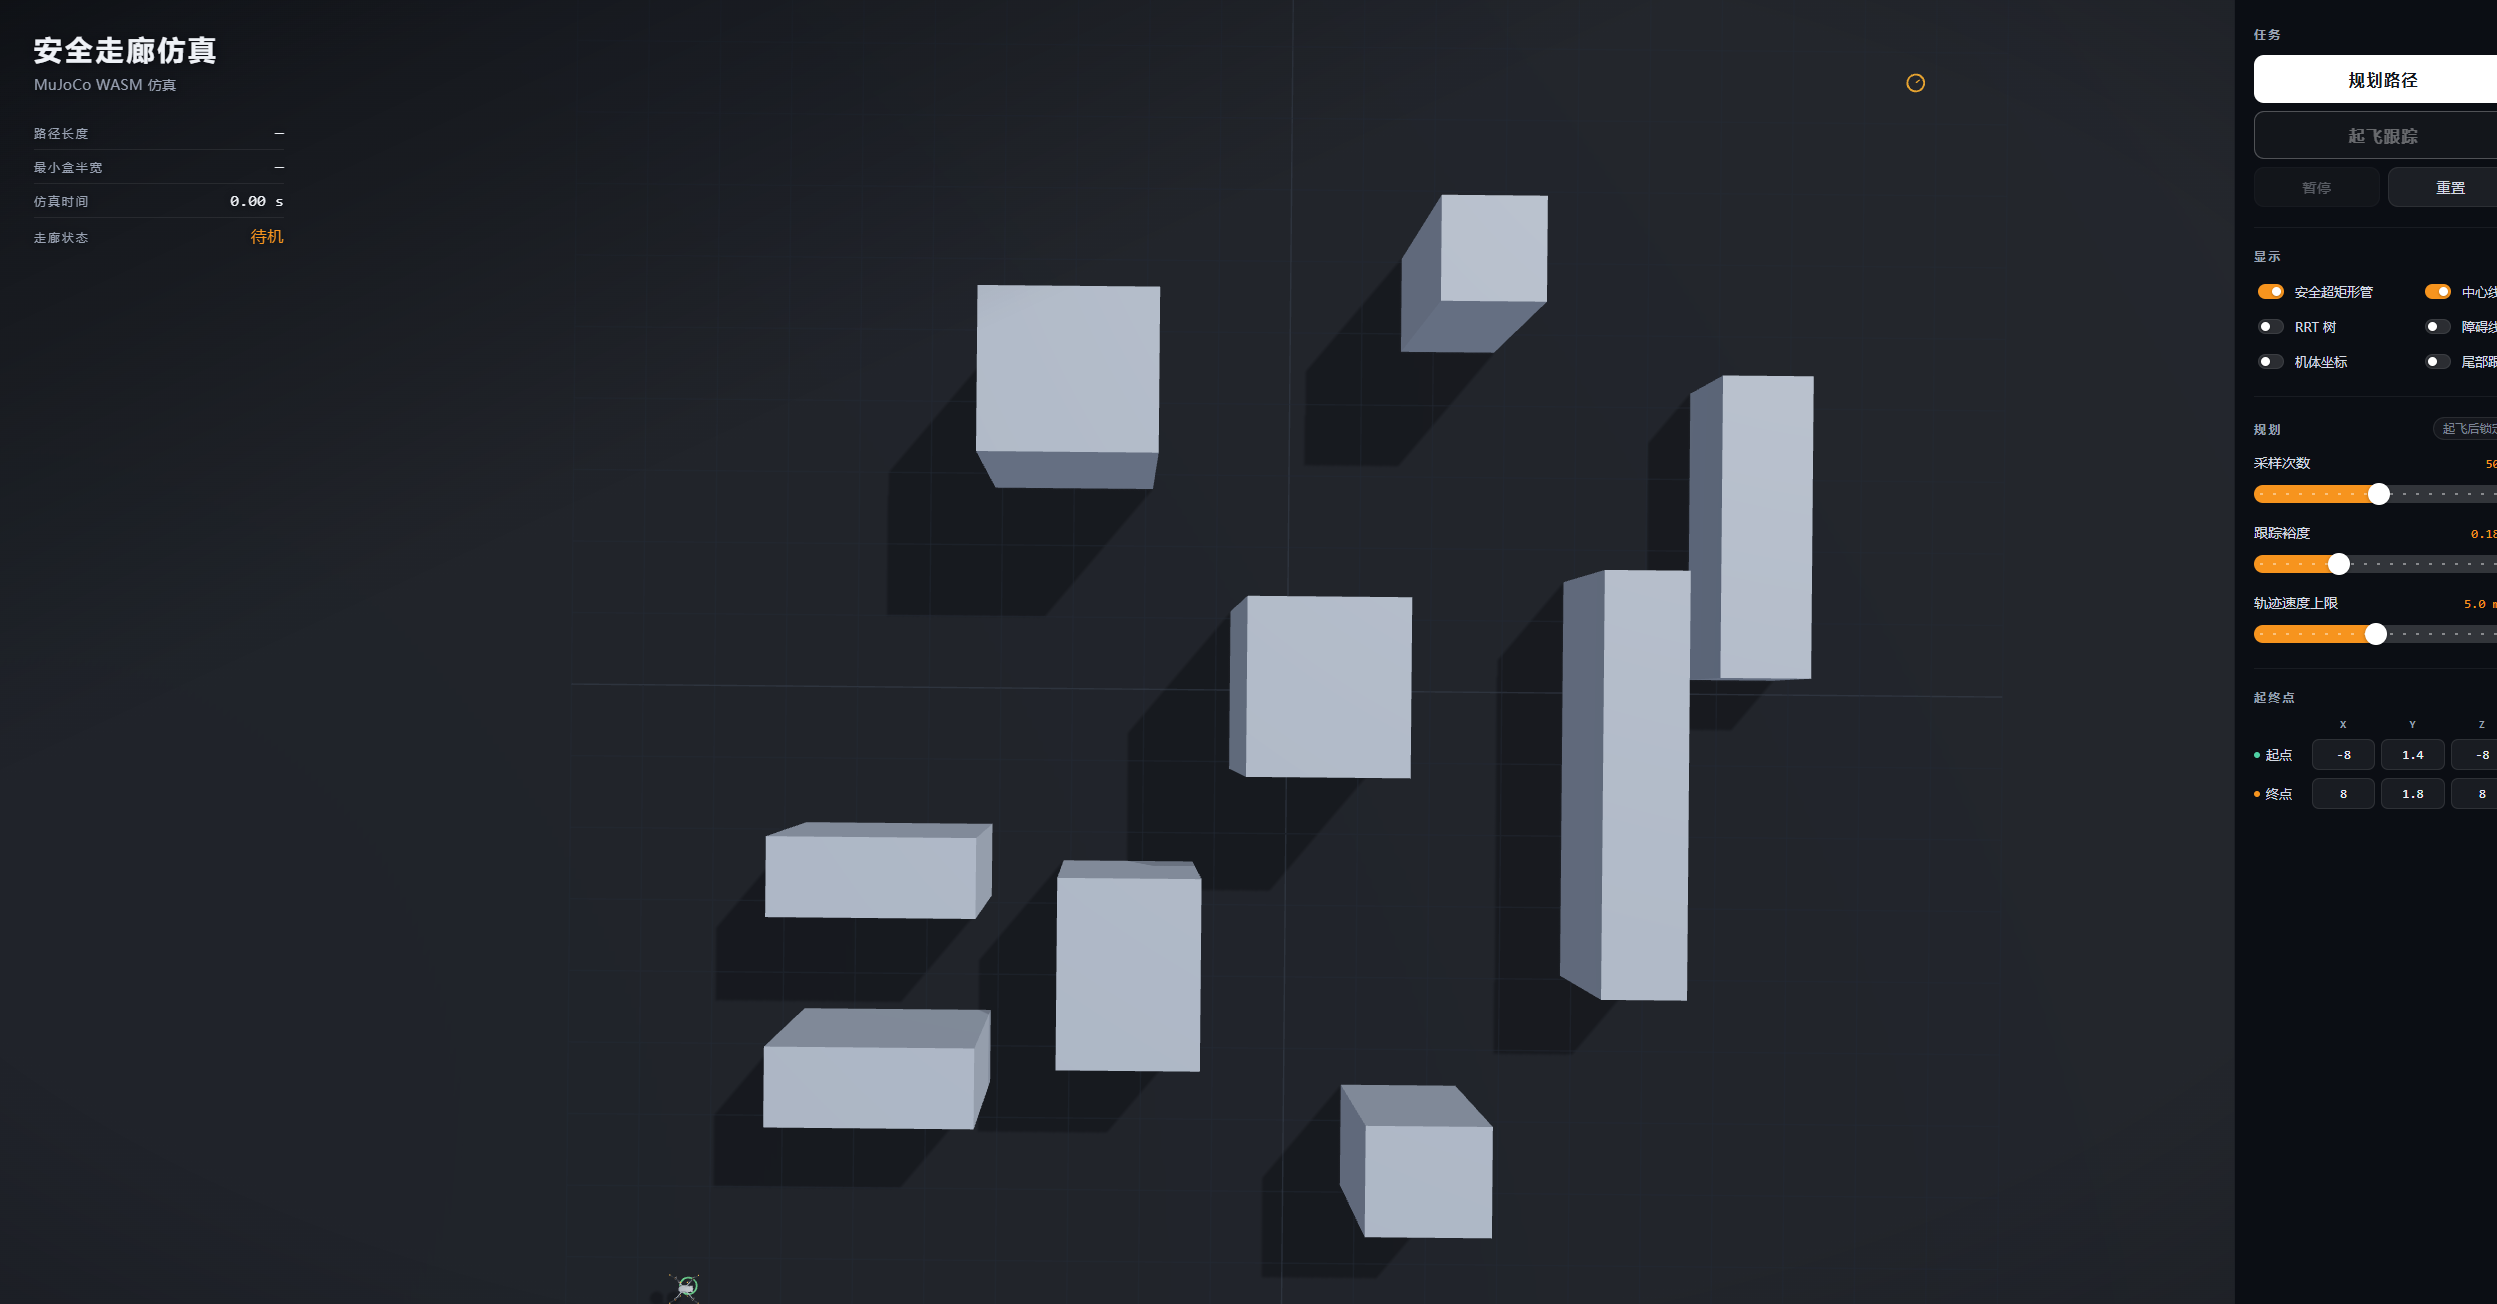
\includegraphics[width=0.96\textwidth]{figures/01-idle-overview.png}
\caption{仿真启动后的俯视场景。左侧 HUD 给出路径长度、最小盒半宽、仿真时间与走廊状态；右侧可调节采样次数、跟踪裕度与速度上限。}
\label{fig:idle}
\end{figure}

点击``规划路径''后，界面进入忙碌遮罩，主线程进行 RRT 扩展与线性规划。一次典型运行得到路径长度 $38.29\,\mathrm{m}$。规划成功后，青绿色超矩形管从起点绕过门柱、矮墙与塔楼连到右上角终点，黄色中心线穿管而过，走廊状态变为``已规划''，如图~\ref{fig:plan}。打开``RRT 树''后，还能看见采样阶段留下的浅色树枝，用以对照最终被保留的那条盒子链，如图~\ref{fig:rrt}。

\begin{figure}[htbp]
\centering
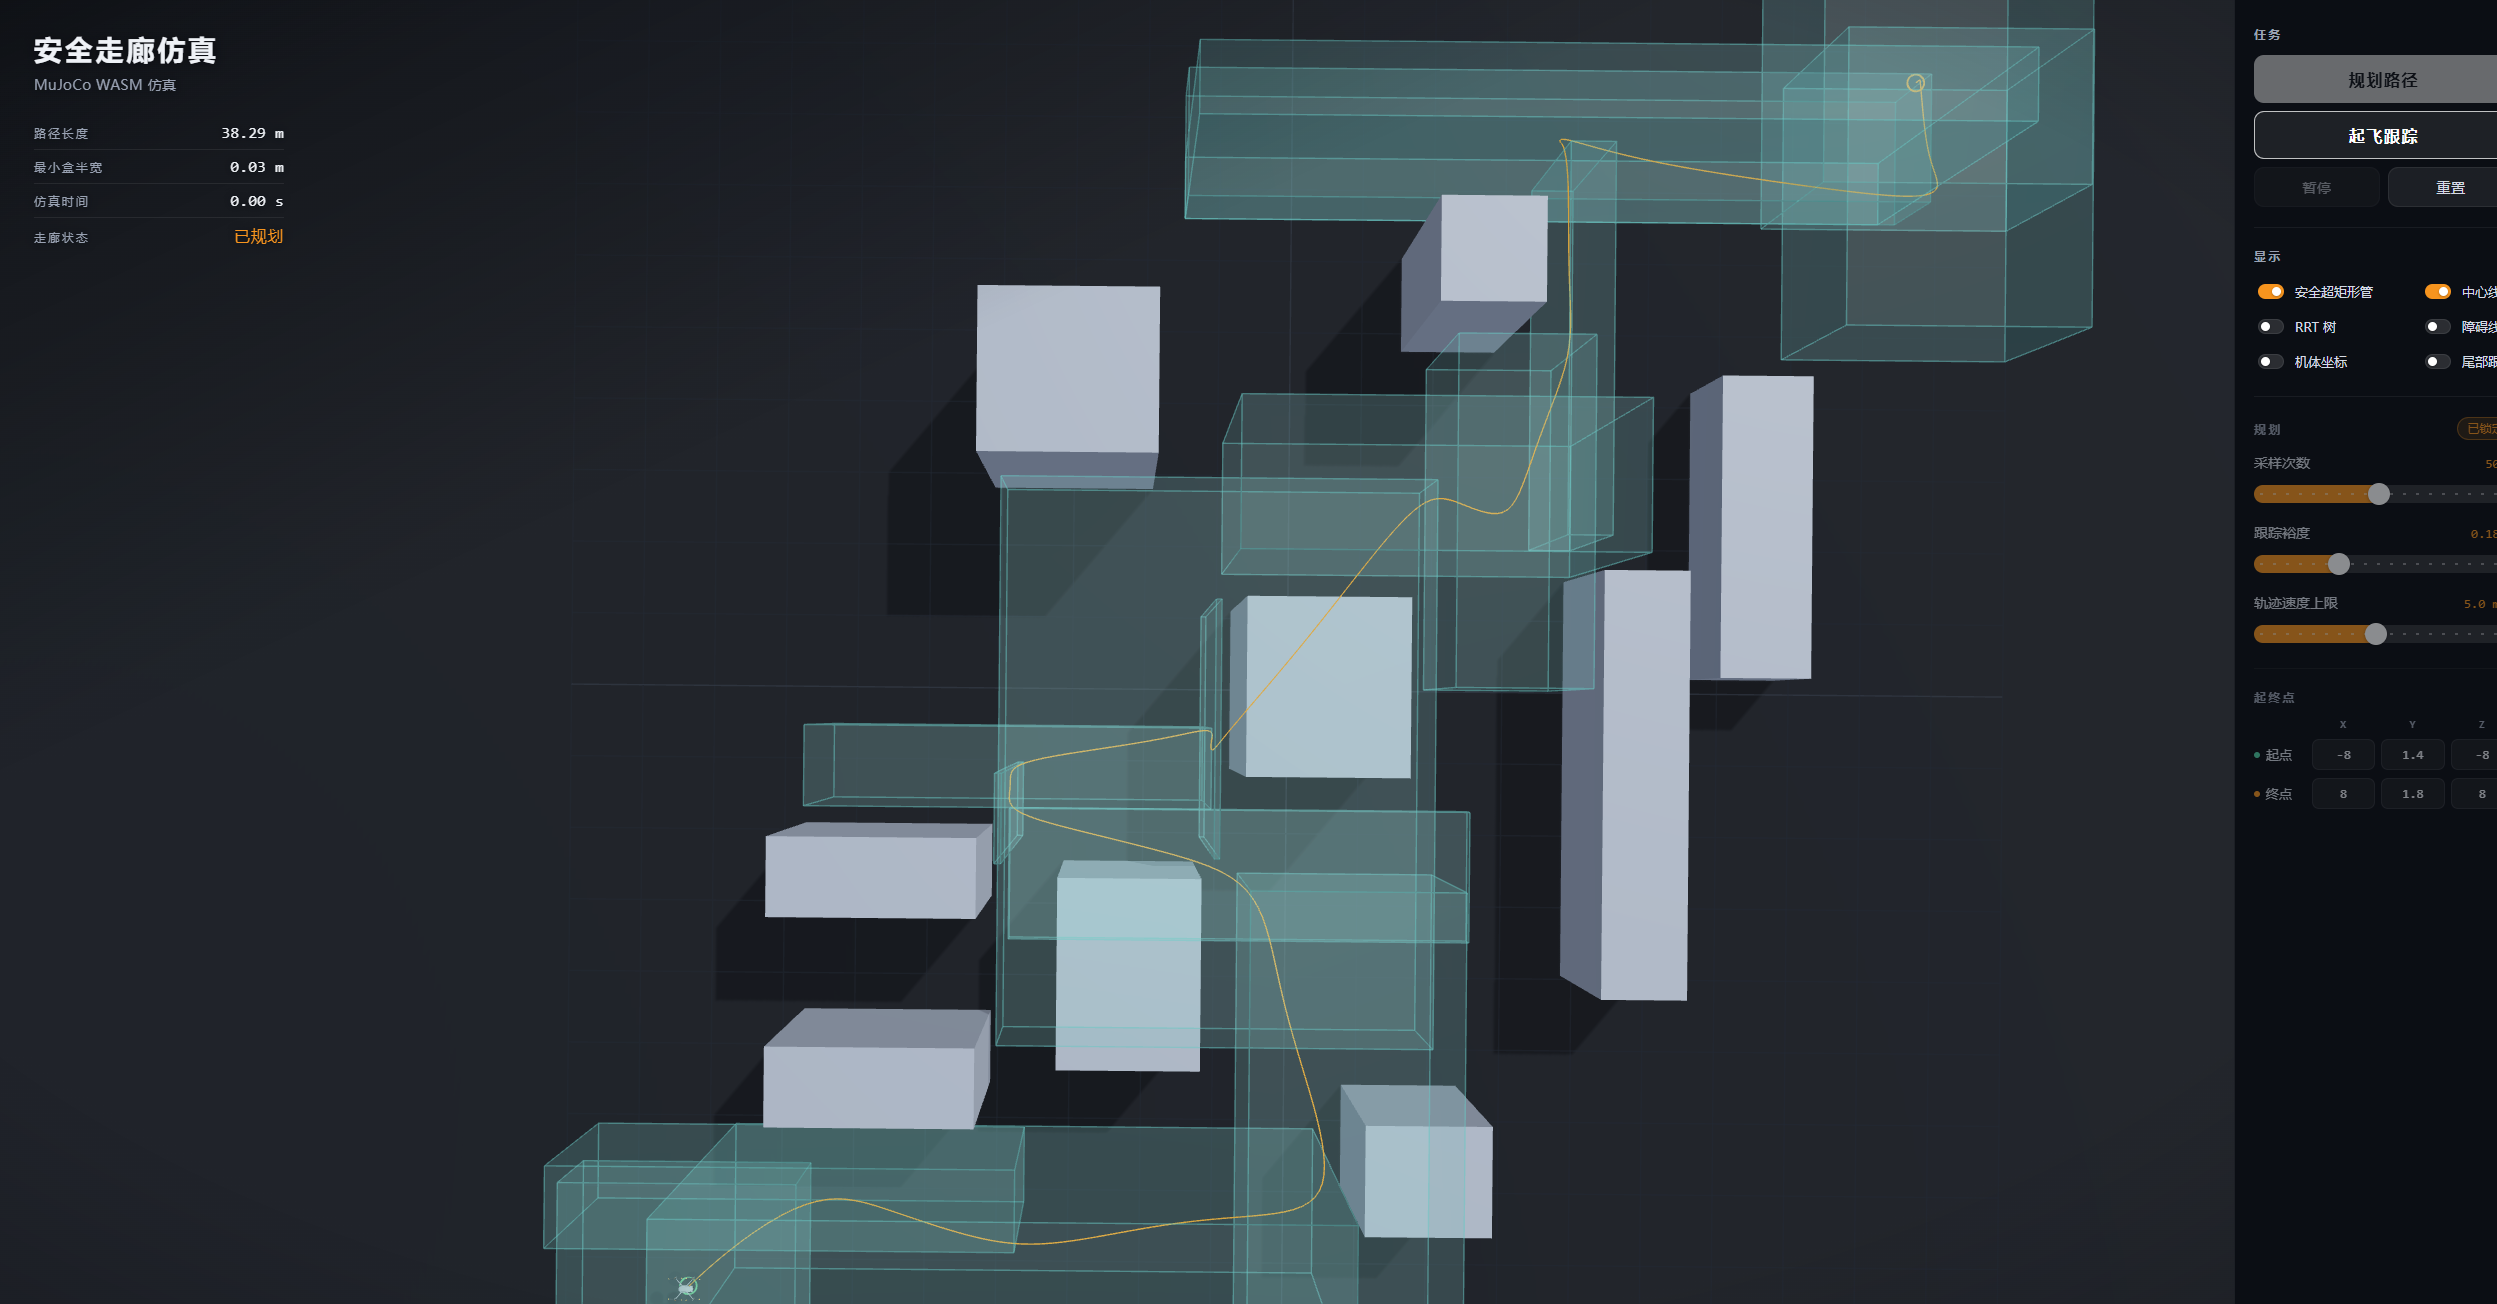
\includegraphics[width=0.96\textwidth]{figures/02-planned-corridor.png}
\caption{规划完成后的安全超矩形管与中心线。起飞按钮此时才可用，避免在无名义轨迹时启动几何跟踪。}
\label{fig:plan}
\end{figure}

\begin{figure}[htbp]
\centering
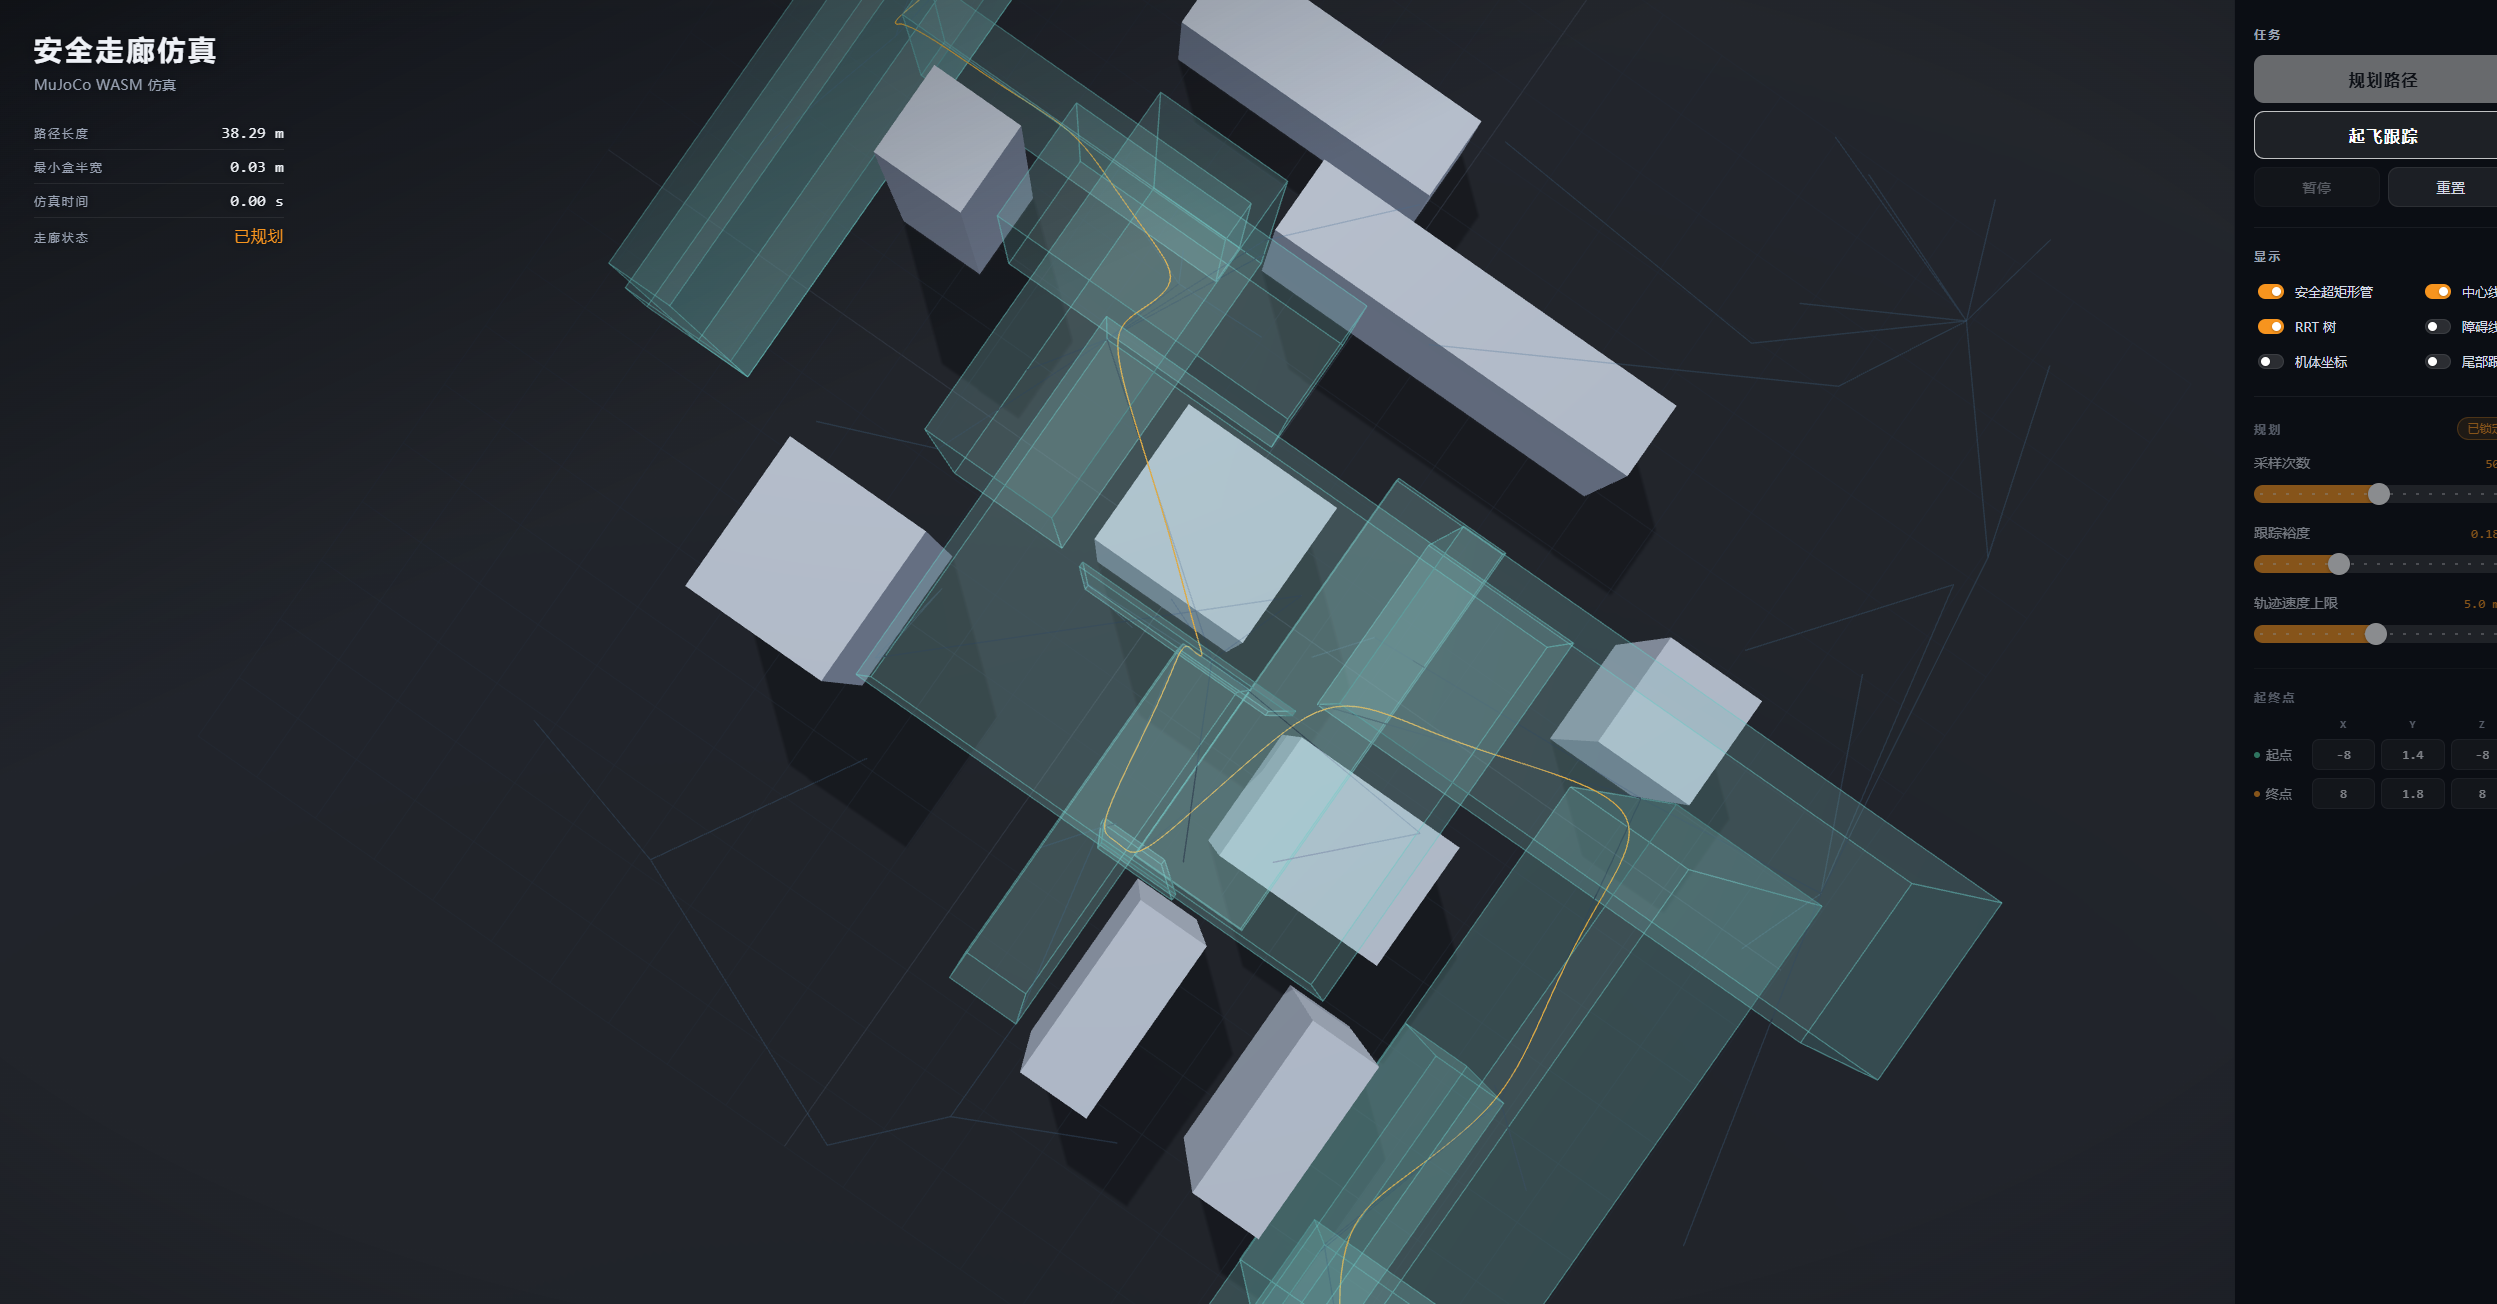
\includegraphics[width=0.96\textwidth]{figures/03-corridor-rrt-tree.png}
\caption{打开 RRT 树显示后的同一规划结果。树展示了采样搜索的覆盖范围，走廊则是从树中提取并经安全矩形计算得到的可行通道。}
\label{fig:rrt}
\end{figure}

点击``起飞跟踪''后，几何控制开始把 MuJoCo 中的自由刚体拉向 B\'ezier 参考。图~\ref{fig:fly} 截取自飞行过程：仿真时间约 $17\,\mathrm{s}$，走廊状态为``管内''，状态栏显示``几何控制跟踪安全管''。再打开``尾部跟拍''，相机落到机体后方，可以看清 \texttt{reference/drone} 的机身、桨叶与管内黄色参考线。机体到达终点后改为定点悬停，图~\ref{fig:follow} 即悬停时刻的跟拍画面，仿真时间约 $92\,\mathrm{s}$，状态为``到达终点，定点悬停''。

\begin{figure}[htbp]
\centering
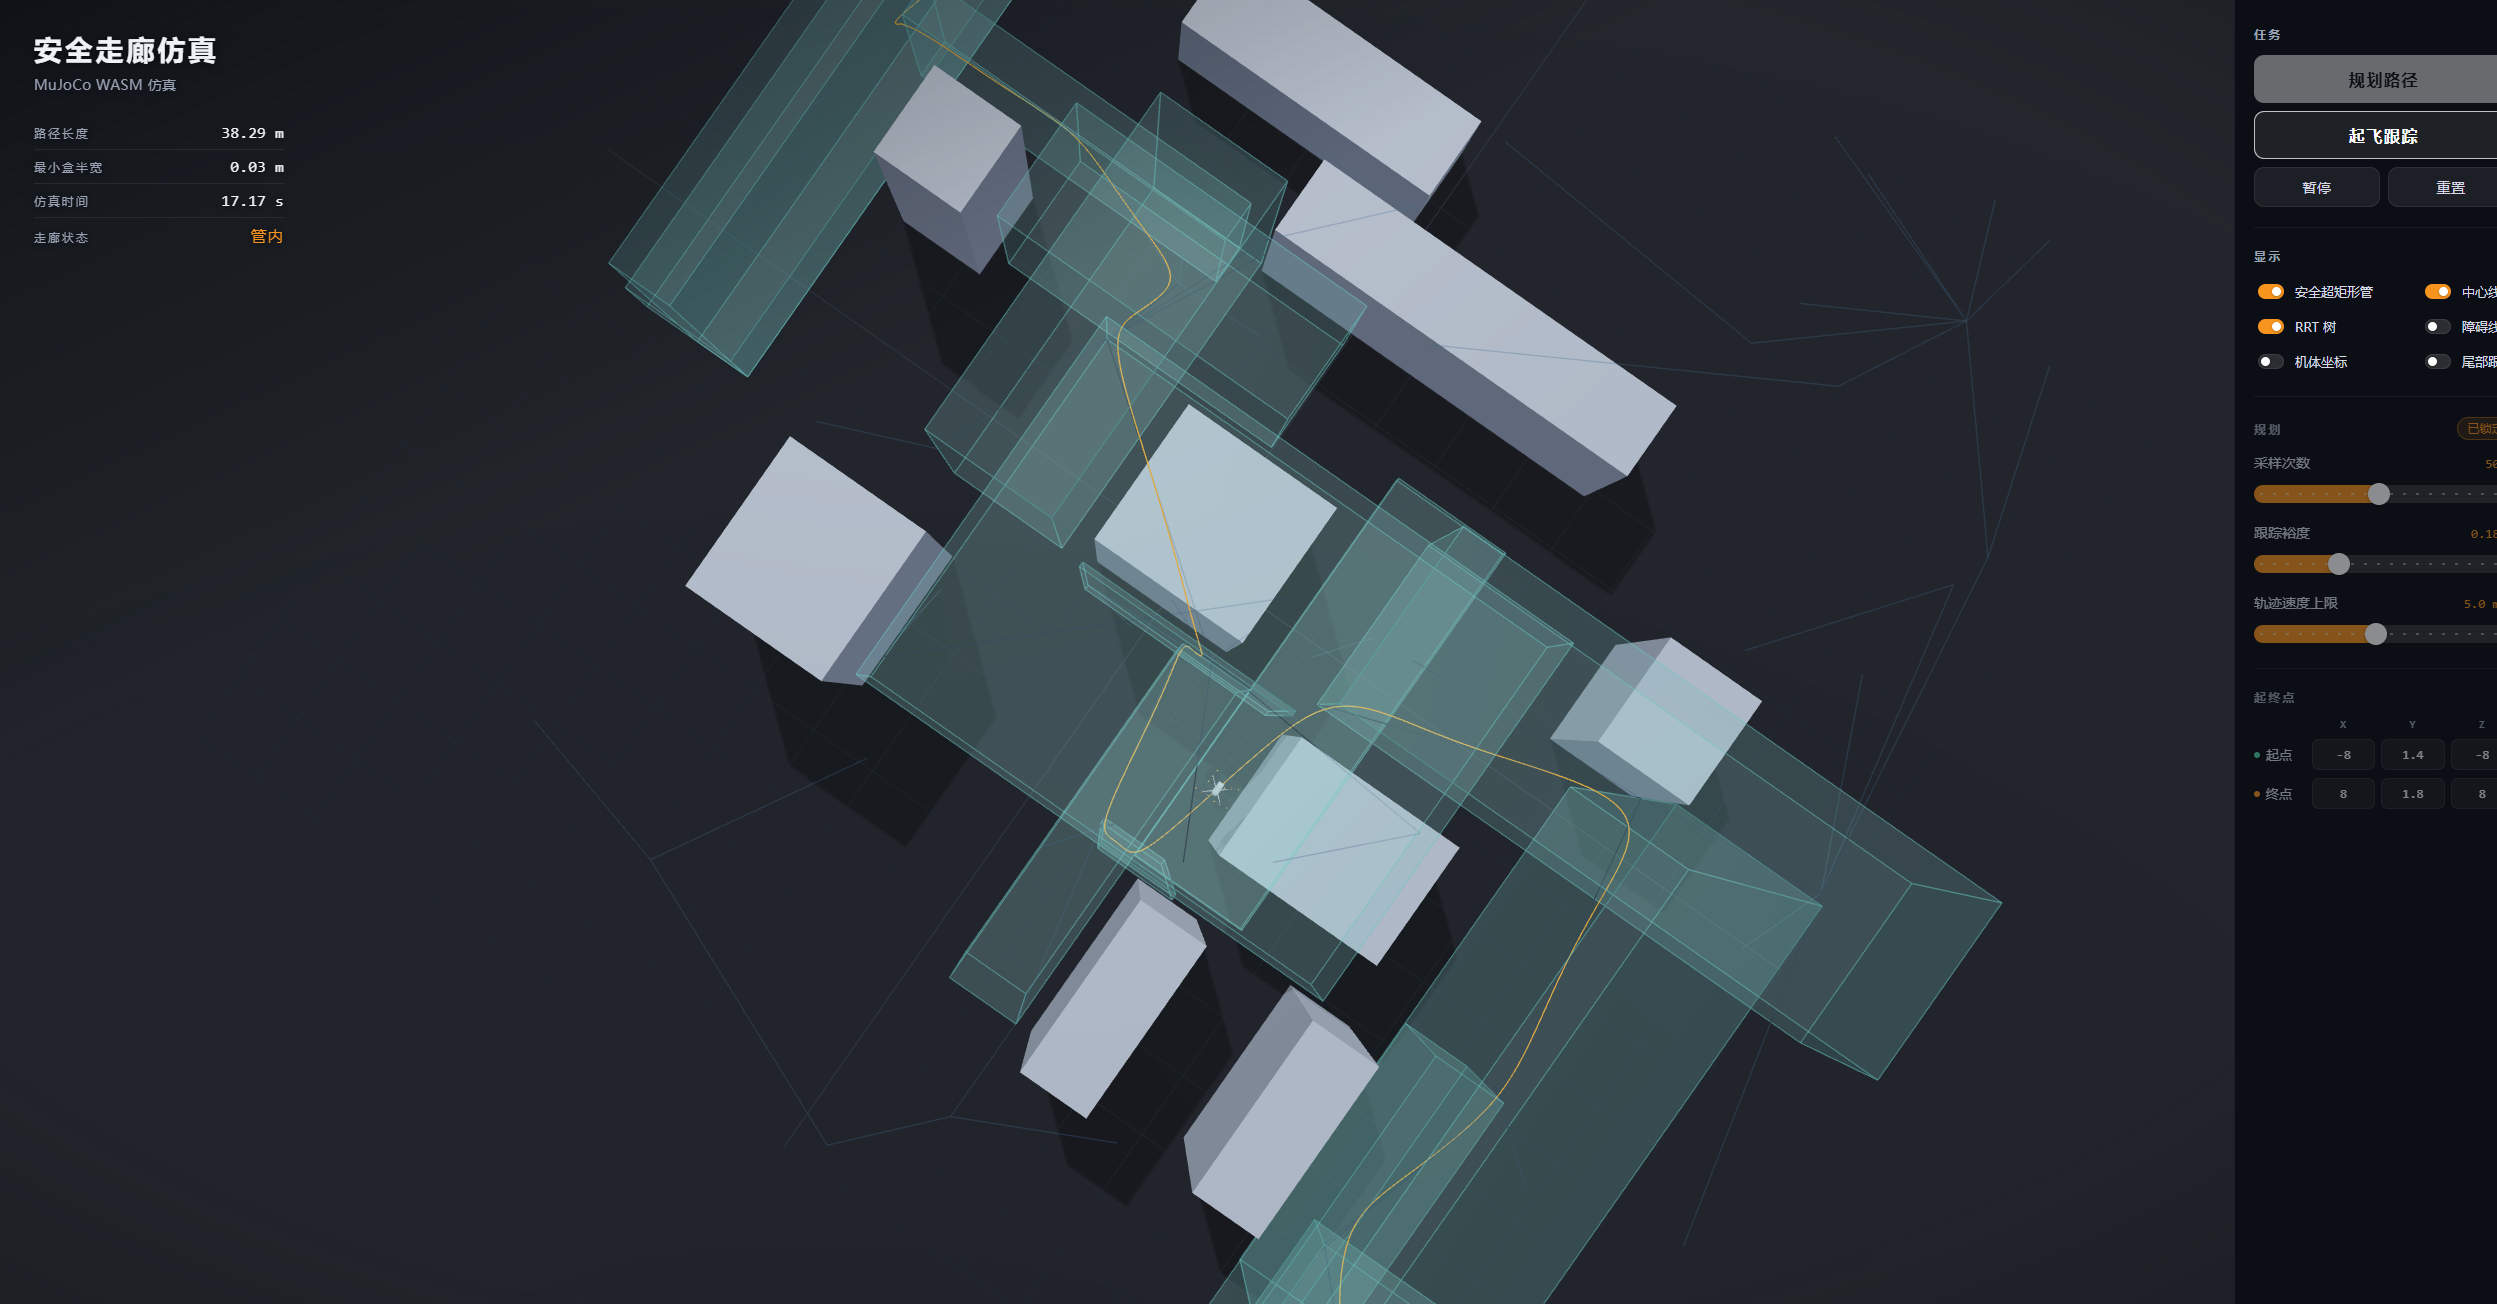
\includegraphics[width=0.96\textwidth]{figures/04-flight-tracking.png}
\caption{几何控制跟踪过程中的俯视。机体沿黄色中心线穿过走廊，HUD 指示仍在管内。}
\label{fig:fly}
\end{figure}

\begin{figure}[htbp]
\centering
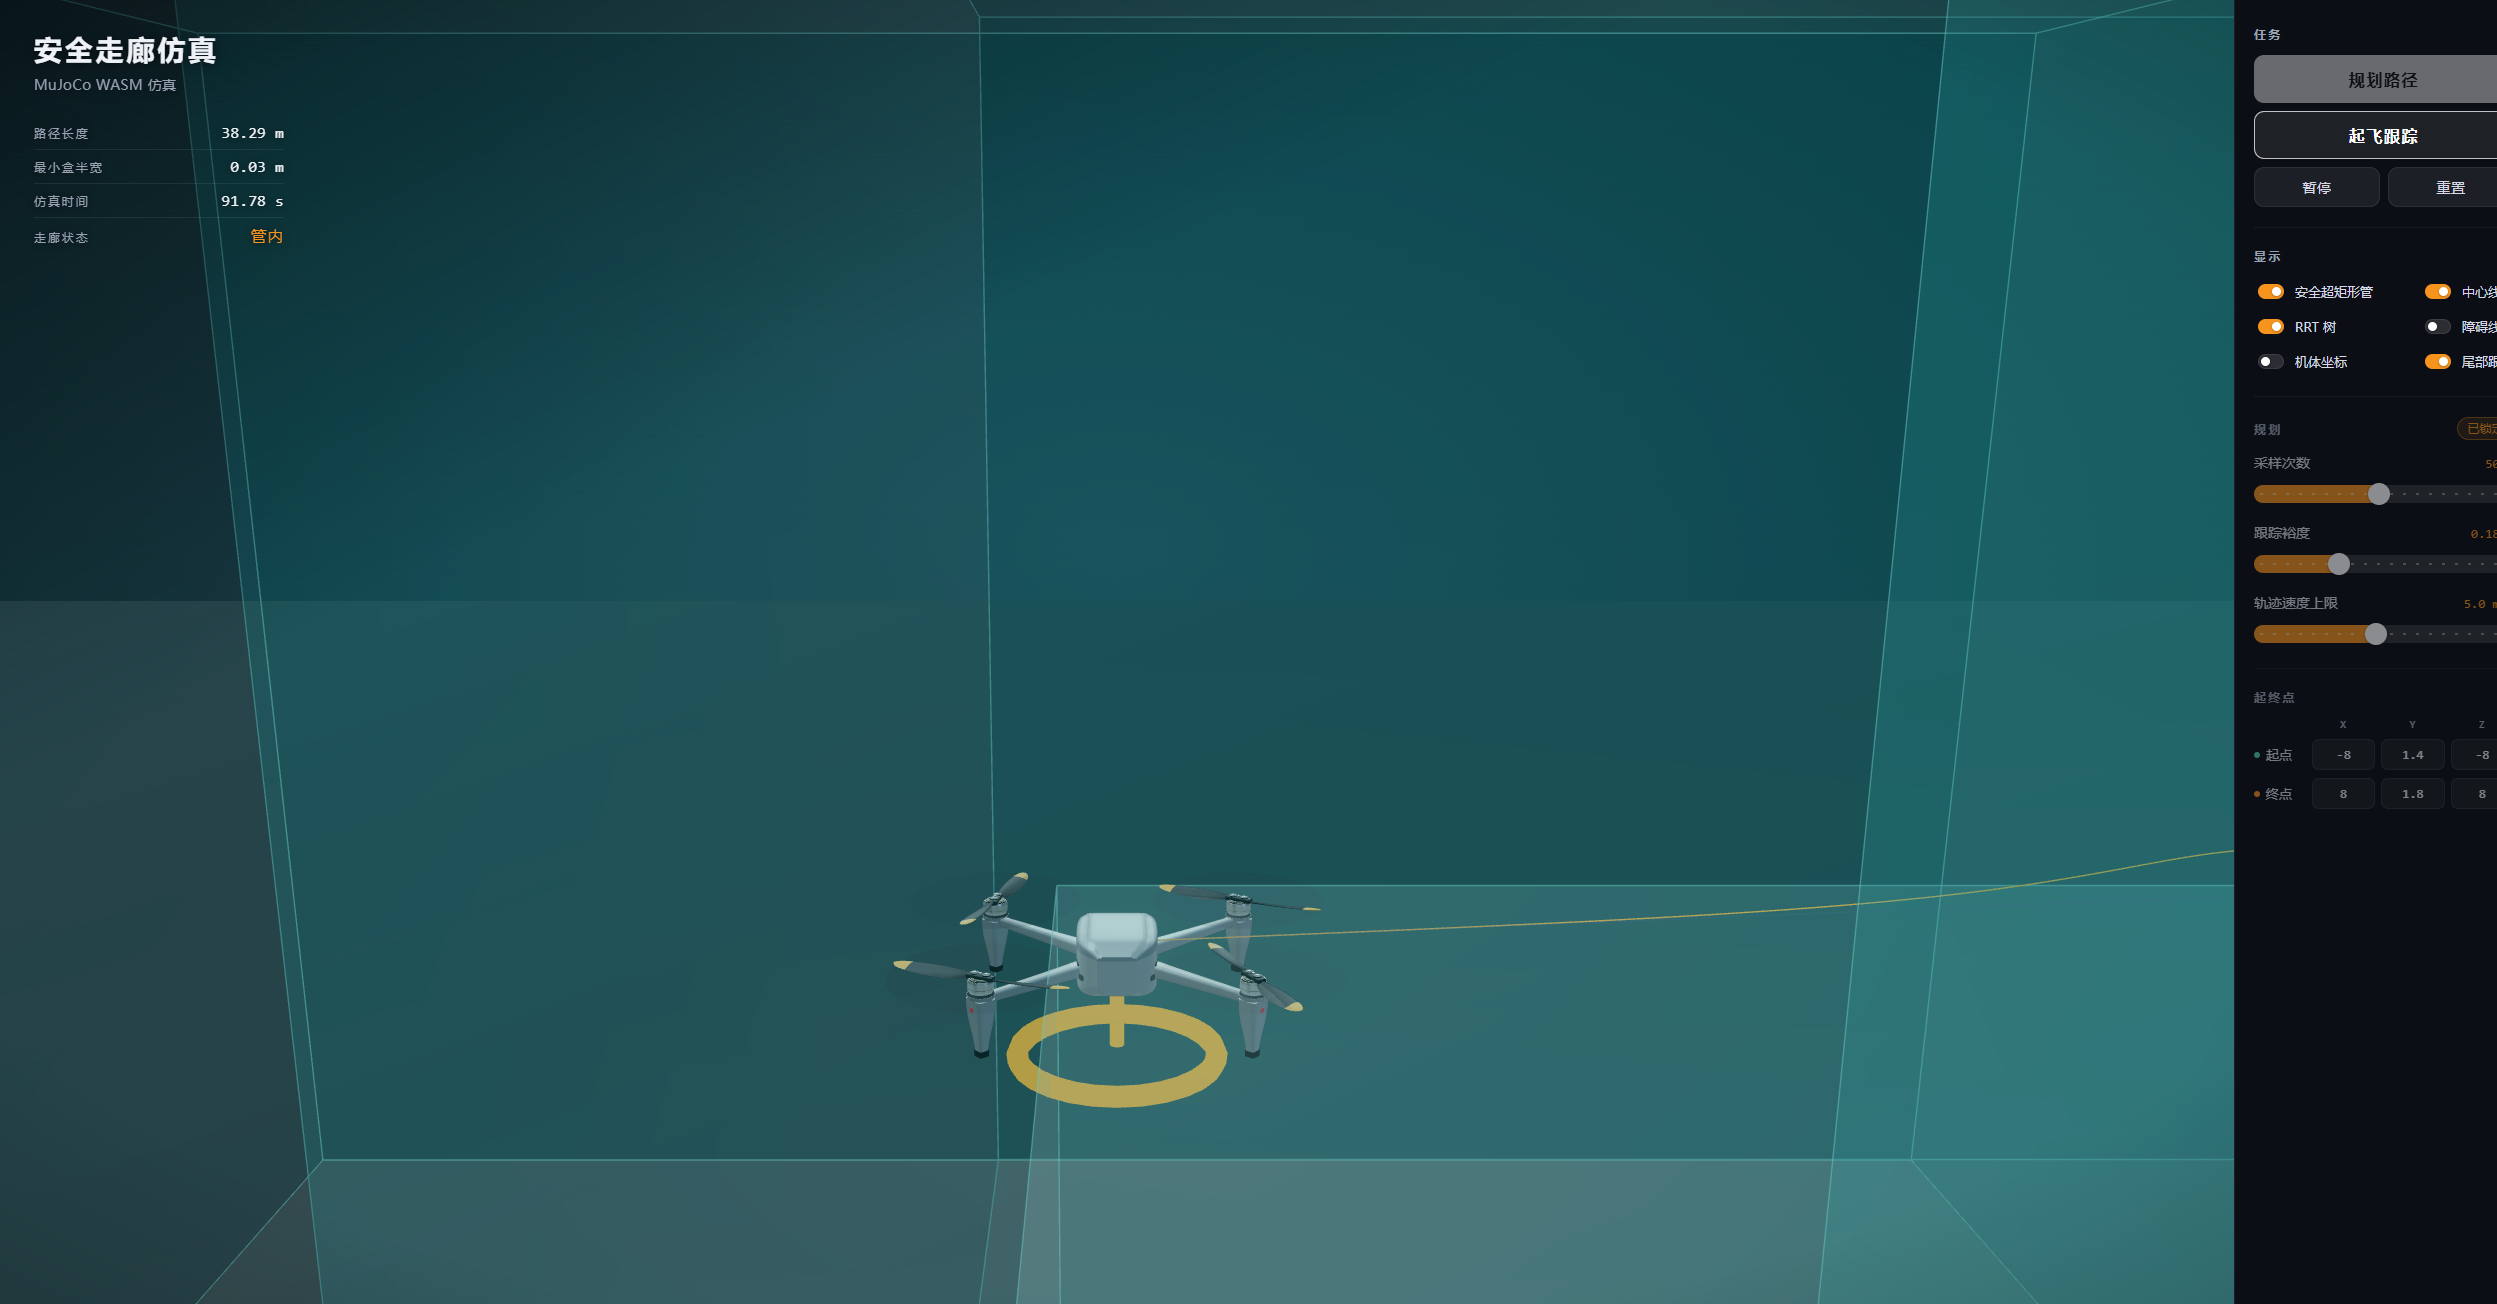
\includegraphics[width=0.96\textwidth]{figures/05-follow-hover.png}
\caption{尾部跟拍视角下到达终点并悬停。半透明走廊盒、中心线与按三视图建模的四旋翼同时可见。}
\label{fig:follow}
\end{figure}

上述操作并未改动默认起终点（起点 $(-8,1.4,-8)$，终点 $(8,1.8,8)$）与默认采样次数 $5000$。交互上还有两点值得记下：规划与飞行期间会锁定起终点和采样滑条，以免中途改参数造成管与控制器不一致；走廊违约不是单帧越界就变红，而是连续若干帧确认后才改写 HUD，避免数值抖动造成误报。

\section{用 Tauri~2 打包桌面程序}
\label{sec:tauri}

网页可以满足演示，但科研现场往往希望``双击即开''。Tauri~2 的官方说明\cite{tauri2}将其定位为：用系统自带的 WebView 构建体积小、启动快的桌面与移动应用，前端可以是任何能编译为 HTML/CSS/JS 的技术，后端按需使用 Rust。与把完整浏览器内核打进安装包的方案相比，Tauri 在 Windows 上使用 WebView2，因而安装包主要包含应用资源而非 Chromium。

\texttt{src-tauri/} 中的配置把产品名设为``安全走廊仿真''，开发期把窗口指到 Vite 的 \texttt{http://localhost:5173}，发布期加载 \texttt{dist/}。为了让 WebView 与浏览器一样能加载 MuJoCo WASM，\texttt{tauri.conf.json} 同样下发 COOP/COEP 响应头。打包目标当前为 Windows NSIS。相关 npm 脚本为 \texttt{npm run tauri:dev} 与 \texttt{npm run tauri:build}。这一层由 Composer~2.5 完成，前端代码无需为桌面单独分叉。

\section{结语}

这篇短文记录的不是又一份``用新框架重写四旋翼仿真''的清单，而是一次把三件事情接起来的实验：MuJoCo 官方 WASM 使物理引擎第一次可以不经本地插件出现在网页里；Three.js 把科研场景从调试 GUI 提升到可演示的三维产品；IEEE TAC 的安全走廊工作\cite{serry2026reachavoid}则为``在障碍中飞过去''提供了比纯几何绕障更硬的安全语义。人机协作在这里的分工也很清楚：人负责把论文读成可做的产品边界，Grok~4.6 铺开前端与算法模块，GPT~5.6~Sol 对着具体失效模式修，Composer~2.5 把同一套页面送进 Tauri 窗口。

当前实现仍是论文方法的工程近似。时变误差界被写成指数裕度，超矩形与 LP 约束针对浏览器算力做了裁剪，碰撞包络是球体而非真实外形。若继续往前走，可以把文献中的闭式界与奇异回避条件更严格地搬进 \texttt{src/plan}，并用脚本批量统计越管率、跟踪误差包络是否被界罩住。那些工作同样适合继续以人机协作的方式进行：人盯住定义是否还叫``安全''，模型负责把定义写成能在 WASM 与 WebGL 里跑起来的代码。

源码与本文所用截图见：
\begin{center}
\url{https://github.com/ZHT1235456/MujocoWASM}
\end{center}

\bibliographystyle{plainnat}
\bibliography{refs}

\end{document}
